%!TEX root = ../masters_thesis.tex

% TODO: all examples as close as possible to the actual domain

\chapter{Basics} % (fold)
\label{cha:basics}

This chapter will lay the theoretical foundation of this Master's Thesis and will embed it into the context of current research. The title of this work is:

\vspace{-1em}
\begin{center}
\textbf{\titleFirst \\ \titleSecond}
\end{center}

It includes the domain (\emph{history of countries}) and the system to acquire, model, manage and visualize data of the domain: \emph{Historical Geographic Information Systems} (HGIS).

The first section of this chapter will define HGIS and related terms. Afterwards, concepts to model time and space in an information system are introduced. Data sources suitable for input into an HGIS are listed in the next section, followed by techniques to manage and analyse the data. A special focus lies on concepts to visualize spatial and temporal data, explained in the next section. The chapter closes with possible HGIS applications and introduces the tool that is used in this thesis: HistoGlobe.


% ==============================================================================
\section{Historical Geographic Information Systems} % (fold)
\label{sec:historical_geographic_information_systems}

\begin{quoteit}
  ``All human actions takes and makes place. The past is the set of places made by human action. History is a map of these places. The past thus exists not in time but in space.''
\end{quoteit}
\hfill -- Philip J. Ethington in \cite[précis]{citeTakeMakePlace}

An Historical Geographic Information System helps to answer research questions about how geographical phenomena have developed over time. To understand how it works, it is important to understand the four parts of the word: The research fields \emph{history} and \emph{geography} and the concepts of \emph{information} an \emph{systems}.


% ------------------------------------------------------------------------------
\subsection{History} % (fold)
\label{sub:history}

History is ``an ideal field for thinking long and hard about important questions''
\cite{ahaFiveCs}.
The Greek word \emph{\textIota\textsigma\texttau\textomikron\textrho\textiota\textalpha / historia}, meaning ``finding out, learning through research, narration of what is learned'', is the origin\footnote{
  \textit{History},
  Dictionary.com, based on Random House Dictionary, 2015,
  URL: \url{http://dictionary.reference.com/browse/history},
  last access: 23.10.2015
}
and it signifies the two main modern usage forms of the term: To research about and learning something and to tell a story. There are many different definitions of the word \emph{history}\footnote{
  \textit{History},
  Merriam Webster -- an Encyclopædia Britannica Company,
  URL: \url{http://www.merriam-webster.com/dictionary/history},
  last access: 23.10.2015
}.
The main goal of history is to study processes in the past to understand the situation in the present and make reasonable decisions for the future. The American Historical Association has developed the ``five C`s of historical thinking [that] together describe the shared foundations of [the] discipline''\cite{ahaFiveCs}:

\vspace{-1em}
\begin{description} % manipulation of indentation
  \item[Change over time]
  The lives of people, their languages and their cultures are continuously changing. Describing these historical changes, triggered by historical events happed in the past, is a major goal of history. Snapshots in the form of historical maps or historical photography are used to tackle this task.
  %TODO: refer to this in later sections
  \item[Context]
  is an important element of historical thinking. The goal is to travel back in time to the moment of the event and recreate the world based on primary sources. The understanding of the historical context is crucial for the understanding of the event.
  \item[Causality]
  The overall goal of each science is to answer the \emph{why}-question concerning an event or a process. For historians that means to reasonably explain an historical event or process based on evidence. The problem is that history is not a science that can alter experimental conditions to extract new information, in a way that e.g. experiments in physics work. Historians have to focus on the interpretation of primary sources, which inherently yields multiple explanations for a single event.
  \item[Contingency]
  is a derived aspect from this problem. Each event has a whole network of prior conditions, because the world is highly interconnected. A slight change in one prior condition could have led to a completely different outcome of the event and a different state of the world.
  \item[Complexity]
  The intrinsic human need for order conflicts with the complexity of history and their events and processes, because of its contingency. It is questionable if all details about events in the world are scientifically explainable.
  %This problem is comparable to the Heisenberg problem in physics: Whereas on the macro-level e.g. physical movements are a direct cause of a set of preconditions (speed, fraction, wind, weight, ...) and are therefore predictable, the smallest of all particles are not traceable, their movements are not predictable and therefore their processes not explainable.
\end{description}

Historical research is conducted by studying and interpreting primary sources, such as written documents, verbal texts, speeches, photographs, audio, video or historical maps. This signifies that most historical research is qualitative. The main organization principle in history is periodization: classifying events and processes to describe broader long-term changes and to explain complex phenomena
\cite[pp.4-7]{knowles2008placing}.
A special focus in this thesis is laid on historical maps as primary source to extract spatial information.

% subsection history (end)

% ------------------------------------------------------------------------------
\subsection{Geography} % (fold)
\label{sub:geography}


The term ``geography'' comes from Greek ~\emph{\textgamma\textepsilon\textomega\textgamma\textrho\textalpha\textphi\textiota\textalpha / geographia}~, literally ``describing the earth.'' \footnote{
  \textit{Geography},
  Dictionary.com, based on Random House Dictionary, 2015,
  URL: \url{http://dictionary.reference.com/browse/geography},
  last access: 23.10.2015
}
It is a science that studies the interplay between the landscapes and environments of the Earth (\emph{physical geography}) on the one hand and the people, their cultures, societies and economies (\emph{human geography}) on the other. That means geography is an interdisciplinary field between natural and social sciences
\cite{rgsGeography}.

Geographical research aims to understand where things are found, why they are there and how they developed over time.
% In regional geography, another subbranch, also the causes of social or environmental differences between cultures and landscapes want to be found.
It focuses on the interconnectivity between elements of physical and human geography, which gets expressed in Tobler's First Law of Geography: ``Everything is related to everything else, but near things are more related than distant things.'' \footnote{
  ``A computer movie simulating urban growth in the Detroit region'',
  Waldo Tobler, 1970
  Economic Geography, 46(2): 234-240.
}

Geographers use different technology and techniques to analyze geographic processes and to answer their research questions. The oldest and most important among those are maps. A map is a graphical expression of something that is not tangible: a part of the real world. A map shows the physical, environmental, political, economical or social properties of the Earth in order for the user of the map to get the most relevant information for his task, may it be orientation, learning or teaching. The ``art and science of making maps'' is the field of \emph{cartography}\footnote{
  \textit{History of maps and cartography},
  James S. Aber,
  URL: \url{http://academic.emporia.edu/aberjame/map/h_map/h_map.htm},
  last access: 24.10.2015
}. Since maps visualize a model, they have a natural constraint: ``No map can perfectly replicate the real world, since it inevitably generalizes, abstracts and approximates the complexity of the reality''
\cite[p. 181]{knowles2008placing}.

% TODO:                 had? had? has had? is having?
% The scientific background of GIS is \emph{geographic information science} (GISci) that studies patterns in natural and human development, e.g. erosion of valleys, literacy rate, natural hazards and deals with approaches and techniques to manage, analyze and visualize this information
% \cite{ngGeography}.


\paragraph{Comparison between geography and history} % (fold)
\label{par:comparison_of_geography_and_history}

Both research fields utilize maps for their research questions, which is the main commonality for the work of this thesis. However, the nature of both fields are also very different, illustrated in table \ref{tab:history_vs_geography}.

\begin{table}[ht]
\begin{center}
\begin{tabular}{p{0px} r c l p{0px}}
    \toprule
    & geography
    & difference
    & history
    & \\
    \midrule
    & where
    & dimension
    & when
    & \\

    & exact, statistical
    & character
    & complex, fuzzy
    & \\

    & mainly quantitative
    & research
    & qualitative
    & \\

    & spatial proximity of conditions
    & causal explanation
    & temporal sequence of events
    & \\

    & spatial differentiation
    & explanation
    & temporal differentiation
    & \\

    & clustering
    & ordering
    & periodization
    & \\

    & mostly visual (maps)
    & expression
    & mostly verbal (texts)
    & \\

    & high (GIS)
    & digitalization potential
    & low (digital humanities)
    & \\
    \bottomrule
\end{tabular}
\caption{differences between history and geography}
\small{\cite[pp. 2-4]{knowles2008placing}}
\label{tab:history_vs_geography}
\end{center}
\end{table}


Whereas geography answers the questions \emph{where?}, history focuses on \emph{when?} -- but the ultimate goal for both sciences is to answer the question \emph{why?}

% paragraph comparison_of_geography_and_history (end)


% subsection geography (end)

% ------------------------------------------------------------------------------
\subsection{Information} % (fold)
\label{sub:information}

The terms ``signs'', ``data'', ``information'' and ``knowledge'' are sometimes used interchangeably and there is no coherent definition for any of them. However, all describe different concepts. This explanation seen in figure \ref{fig:information} is based on the work of \cite{datinfwis}.

\begin{figure}[ht]
  \vspace{1em}
  \begin{center}
    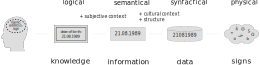
\includegraphics[width=0.9\textwidth]{graphics/basics/information}
  \end{center}
  \caption{signs, data, information and knowledge}
  \label{fig:information}
\end{figure}

A \emph{sign} is the physical representation of something in the real world. Since the real world is continuous, literally anything can be seen as a sign, so there are uncountably infinitely many different signs. \emph{Data} is a subset of all possible signs and represents the syntactical level of what an information system deals with. Data itself does not have any meaning, but as soon as it is organized, it becomes \emph{information}. However, information is sensitive to its cultural context. The string ~\texttt{14.07.1789}~ is useful and understandable for people in countries that use the date format \texttt{DD.MM.YYYY}. However, for people in Belize and the USA, that use the format \texttt{MM.DD.YYY}, this might just be a random string of numbers without any meaning, and therefore no information -- although it is the same data. If information is visualized to and understood by a human and it can be integrated into his or her larger subjective context, it is \emph{knowledge} \cite{nake}. The goal of a visualization is to present as much information as possible in a way that it can be transformed into knowledge by the viewer.

% subsection information (end)

% ------------------------------------------------------------------------------
\subsection{System} % (fold)
\label{sub:system}

A \emph{system} is an organized structure containing \emph{elements} or \emph{components} that are directly or indirectly \emph{related} to and \emph{interconnected} with each other. The elements and their relations form the whole of the structure. The surrounding of the system is its \emph{environment}. There is an \emph{internal state} at any point of the system's existence. This state only changes when it gets influenced by stimuli of its environment. \emph{Emergent properties} characterize a system. They are independent from properties of the element of the system, e.g. water is liquid at room temperature, but the elements it consists of, hydrogen and oxygen, are a gas. Each system is both part of a larger system and can be decomposed into subsystems. Therefore, systems form a hierarchy.

A system has defined spatial and temporal boundaries. There are two types: \emph{open systems} allow exchange of energy or information with their environment, whereas idealized \emph{close systems} naturally do not interact with and are not influenced by its environment. Based on the black box principle the inner working of a closed system can not be seen from the outside
\cite{system}.

% subsection system (end)

% ------------------------------------------------------------------------------
\subsection{Definition and Motivation} % (fold)
\label{sub:definition_and_motivation}

An \emph{information system} (IS) is an application that is dealing with the acquisition, management, analysis and presentation of information. It is the unity of all its components and their interaction with each other
\cite{informationSystem}.
If the majority of the information in a system has a spatial relation to the Earth, its surface, its lithosphere, atmosphere or the social or economical structure of its habitation, it is a \emph{geographic information system} (GIS). The data objects in the system are called \emph{geo-objects}
\cite{bolstad2008gis}.
If the information additionally has a temporal dimension, e.g. via time stamps or time spans, which enable to trace developments of geo-objects, it becomes an \emph{temporal} or \emph{historical geographic information system}.
\cite{gregory2014toward}.

HGIS react on the spatial turn of history: the integration of geographic methods in historical research. It aims to discover the power of cartographic representation: ``The spatial turn in the humanities must [...] understand the role of space in human events''
\cite{bodenhamer2010spatial}.
At the same time, they are the product of the temporal run in GIS: the coexistence of space (where things are) and time (what has changed over time)
\cite[p. 45]{solana2014spatio}.
With HGIS it is possible to analyze how ``spatial patterns change over time in order to better understand large-scale Earth processes''
\cite{peuquet99}.
Since ``the world never stands still'', but ``the retention of information relating to past events [is] an important element of human representation of the world'', the dimension of time has to be integrated into a GIS
\cite{peuquet99}.

Historical Geographic Information Systems consist of mainly four components: The acquisition part describes everything that is related to the input of \emph{spatio-temporal data}. It is physically stored and logically managed in a \emph{spatio-temporal database}. It will be analyzed regarding different aspects of the task in order to make sense of them: Transforming them into information that can be used to answer the question of the user. The resulting information will be presented on a display suited for space (e.g. a map) and time (e.g. a timeline). From the visualization the viewer can extract \emph{spatio-temporal knowledge}. All components will be explained in more detail in this chapter.

HGIS are also called \emph{Spatio-Temporal Information Systems} (STIS)
\cite{pelekis04stdms}.

% subsection definition_and_motivation (end)

% section historical_geographic_information_systems (end)


% ==============================================================================
\section{Modelling Time and Space} % (fold)
\label{sec:modelling_time_and_space}

A model tries to replicate a part of the real world. A data model abstracts a part of the world, identifies the most essential elements and their relation to each other and conceptualizes them e.g. in an \emph{Entity Relationship Model}. In an HGIS, the data model should contain entities and relations to explain spatial-temporal phenomena in the real world. Based on the theory of the \emph{Triadic Framework}, there are three components involved: space (3 dimensions), time (1 dimension) and attribute (multiple dimensions). All of these dimensions can change independently from each other
\cite[p. 53]{ott2001time}.

% TODO: absolute time vs. relative time
% TODO: absolute space vs. relative space

The remaining part of the section will introduce ways to separately represent time and space in an information system.



% ------------------------------------------------------------------------------
\subsection{Representation of Space} % (fold)
\label{sub:representation_of_space}

The information system needs to unambiguously locate each geo-object on, underneath or close to the Earth's surface using \emph{geographic coordinates}. They allow to locate an object directly in the coordinate system of the geodetic datum. In order to do that, a geo-object has to be expressed in the coordinate system of the Earth.

% ------------------------------------------------------------------------------
\subsubsection{Geospatial Data Model} % (fold)
\label{ssub:geospatial_data_model}

To model the Earth in an information system, its actual shape has to be analyzed. It is measured by scientists in the field of \emph{geodesy} is rather complicated. In the Babylonian Empire ($\approx$ 2000-539 BC) the theory of the Earth being a flat disc surrounded by an infinite body of water
%(a theory still valid in some southern parts of the United States of America)
evolved. The Greek scientists Pythagoras and Aristotle (340 BC) rejected this theory and proved the earth to be a three-dimensional spherical object. It took almost 2000 years until Sir Isaac Newton (1687) reasoned that due to the centrifugal forces of the rotating Earth the shape has to flattened at the poles and is therefore better described as an \emph{ellipsoid} with two radii: the polar radius ($r_p$) and the slightly larger equatorial radius ($r_e$)
\cite[pp. 69-77]{bolstad2008gis}.

However, the model disregards that the surface of the Earth is not flat but consists of deep oceanic trenches and high mountains. Therefore the gravitational field of the Earth is not homogeneous either: the actual \emph{mean sea level}, the reference surface for the height ofgeo-objects from 106 meter below to 85 meter above the uniform sea level of the ellipsoid model. These discoveries in the \nth{20} century led to the complex \emph{geoid} model (see figure \ref{fig:geoid}). The latest and most accurate measurements for the shape of the Earth are the result of the GOCE satellite launched in March 2009
\cite{geoid, geoidESRI}.

\begin{figure}[H]
  \centering
  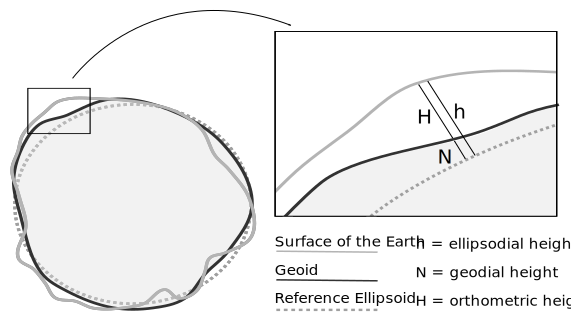
\includegraphics[width=0.66\textwidth]{graphics/basics/geoid}
  \caption{The geoid model, differences are exaggerated}
  \small{based on \cite[Fig. 3-6, p. 75]{bolstad2008gis}}
  \label{fig:geoid}
\end{figure}


\paragraph{Geographic coordinate system} % (fold)
\label{ssub:geographic_coordinate_system}

The reference ellipsoid is the basis for the model that is used to determine an object's position relative to the Earth's surface. It is represented in a three-dimensional \emph{spherical coordinate system}.

This ellipsodial model defines the \emph{North Pole} and the \emph{South Pole} as the two surface points closest to the Earth's center and the \emph{Equator} as the line equidistant to the two poles and therefore dividing the world in a \emph{Northern} and \emph{Southern Hemisphere}. Additionally, the \emph{Prime Meridian} is defined as the line perpendicular to the Equator, running from the North to the South Pole. Since there are infinitely many lines like this, its definition is arbitrary, but by convention, the line running through Greenwhich, London, United Kingdom is used.

Based on these two lines, each point in the spherical coordinate system can be unambiguously defined by three values
(see Figure \ref{fig:geo-coordinates}):

\begin{enumerate}
  \item The rotation angle along the Equator, defining its longitude: $\gamma = [-180\degree ~...~ +180\degree]$
  \item The rotation angle along the Prime Meridian, defining its latitude: $\phi = [-90\degree ~...~ +90\degree]$
  \item The distance to the origin: $r \in \mathbb{N}_0$
\end{enumerate}

\begin{figure}[ht]
  \vspace{1em}
  \centering
  \includegraphics[width=0.8\textwidth]{graphics/basics/geo-coordinates}
  \caption{Geo-coordinates using latitude and longitude}
  \small{based on \cite[pp. 26-28]{bolstad2008gis}}
  \label{fig:geo-coordinates}
\end{figure}

Lines of constant latitude are running horizontally and are called \emph{parallels}, lines of constant longitude are \emph{meridians} appearing in vertical direction. All parallels are circles with their center on the axis between the poles. No two parallels intersect. The longest parallel is the Equator (0\degree~latitude). All meridians have the same length.

Geographic coordinates are usually recorded either in degree-minutes-second (\texttt{DMS}, e.g. \texttt{50\degree~58' 22''}) or in decimal degree (\texttt{DD}, e.g. \texttt{50.973}) notation
\cite[pp. 30, 79]{bolstad2008gis}.


\paragraph{Geodetic datum} % (fold)
\label{par:geodetic_datum}

One main task of a GIS is to accurately visualize the Earth on a map. Since the Earth is an inhomogeneous three-dimensional shape but the output medium is a two-dimensional computer screen or piece of paper, it has to be transformed. First the Earth has to be modeled using the \emph{geodetic datum}. It consists of two parts: The approximation of the Earth's surface in a the Cartesian coordinate system with the origin and a set of reference points used to accurately locate a point.

Geodetic datums can be very accurate in one region of the world, i.e. the model fits the real geoid very well, but inaccurate in another region. This is the main reason why there are a lot of different geodetic datums used in the world. The same coordinates in two different geodetic datums define two different points on Earth. In order to be accurate is essential to know the geodetic datum of the coordinates
\cite[p. 80]{bolstad2008gis}.

The \emph{World Geodetic System 1984 (WGS84)} is a model that found worldwide acceptance and is used in all major Web-based mapping services like \emph{OpenStreetMap} and is implemented in the GPS unit of all major smart phones.

% paragraph geodetic_datum (end)

% subsubsection geospatial_data_model (end)

% ------------------------------------------------------------------------------
\subsubsection{Raster and Vector Model} % (fold)
\label{ssub:raster_vs_vector_model}

Geographical features like cities, houses or country borders are infinite in detail. But storage in a computer system is finite. In order to model these continuous phenomena in an information system, a relevant subset of them has be sampled to create discrete spatial data. It can be represented in a raster or in a vector model.

\begin{figure}[H]
  \centering
  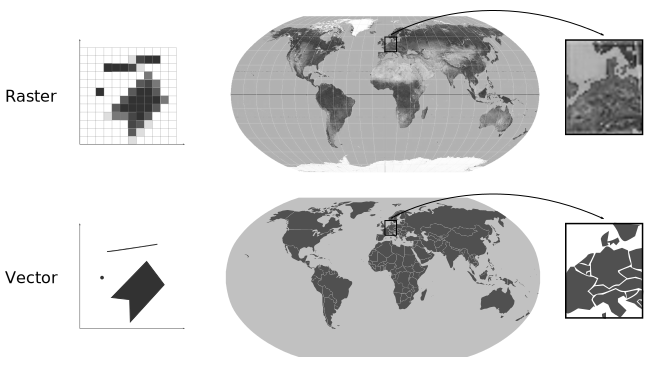
\includegraphics[width=0.8\textwidth]{graphics/basics/raster_vector}
  \caption{Comparison of the raster and the vector model}
  \label{fig:raster_vector}
\end{figure}

The \emph{raster model} contains a regular grid with a fixed \emph{cell dimension}. Each cell has a certain value, e.g. a color value, height or population density.
The raster model is simple and allows straightforward rendering: only affine transformations have to be applied in order to project e.g. two raster map layers on top of each other. The main disadvantage of the raster model is its fixed resolution: it can not be scaled up without losing quality
\cite[pp.42-48]{bolstad2008gis}.
Raster graphics are used by most map engines for the basic map layer in form of map tiles, e.g. in OpenStreetMap or the satellite image of the Earth by NASA in Google Maps.
% \footnote{
%   \textit{Google Maps},
%   URL: \url{https://www.google.com/maps/@51.2090662,13.2328189,3563505m/data=!3m1!1e3},
%   Imagery \textcopyright2015 Landsat, Data SIO, NOAA, U.S. Navy, NGA, GEBCO, IBCAO, U.S. Geological Survey, Map data \textcopyright2015 Google, ORION-ME,
%   last access: 29.10.2015
% }.

In the two-dimensional \emph{vector model}, each object is a mathematically described geometric primitive. There are three basic primitives (figure \ref{fig:geometric_primitives}):

\begin{figure}[H]
  \centering
  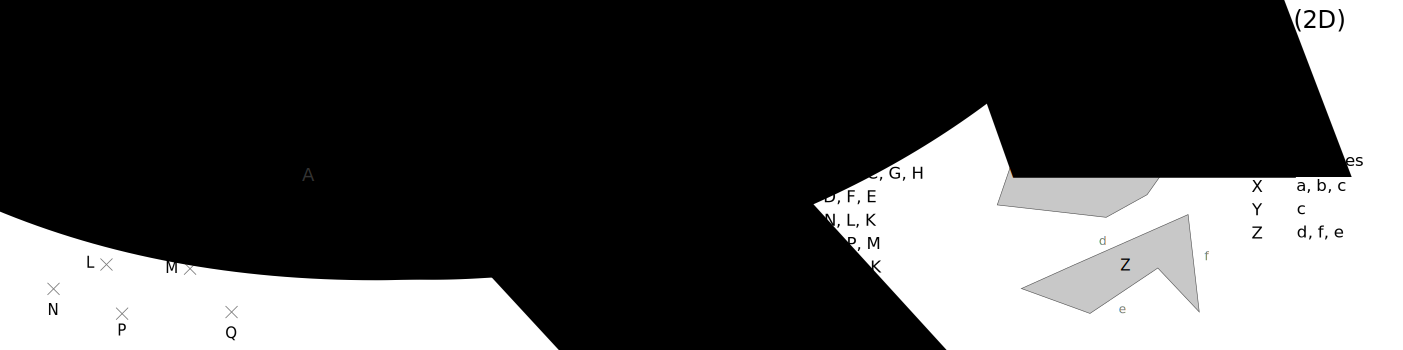
\includegraphics[width=0.65\textwidth]{graphics/basics/geometric_primitives}
  \caption{The basic geometric primitives point, polyline and polygon}
  \label{fig:geometric_primitives}
\end{figure}

\begin{enumerate}
  \item[0D] A \emph{point} is the fundamental object in vector geometry. It has no dimension, no size and is only defined by its position, specified in geographic coordinates. One point is independent from all other ones. Points can be used e.g. to represent a landmark.
  \item[1D] A \emph{polyline} is constructed by an ordered set of points with at least one start and one end point. A street can be expressed by a polyline.
  \item[2D] A \emph{polygon} is an ordered set of polylines creating a closed area. A polygon can be \emph{simple}, \emph{weakly simple} or \emph{complex} (see figure \ref{fig:polygon_properties}). A lake can be described by a polygon.
\end{enumerate}

Additionally, a \emph{polypolyline} represents multiple separate lines belonging to one logical entity, e.g. an interrupted highway. In the same way, a \emph{polypolygon} describes the union of multiple separate areas, e.g. a set of islands of an archipelago.

\begin{figure}[H]
  \centering
  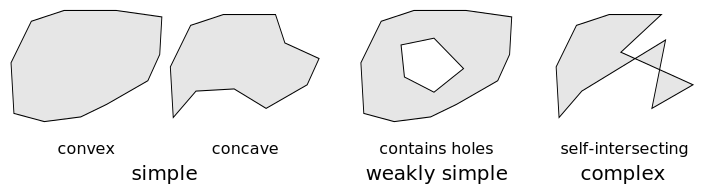
\includegraphics[width=0.8\textwidth]{graphics/basics/polygon_properties}
  \caption{Different properties of polygons}
  \label{fig:polygon_properties}
\end{figure}

Scale-independence is one of the biggest advantages of a vector model. The data model is more compact in comparison to the raster model. On the other hand, the model can become very complex. Since vector data has to be rasterized to be shown on the screen, the computational effort increases with complexity \cite[pp.33-42]{bolstad2008gis}.

Vector models are suitable to represent phenomena in real world that can easily to discretized, e.g. the boundaries of a national park. Common file types for vector data with spatial reference are the open file formats GeoJSON (\texttt{.geojson})\footnote{
  \textit{GeoJSON},
  IETF Geographic JSON Working Group,
  URL: \url{http://geojson.org/},
  last access: 30.10.2015
}
and Scalable Vector Graphics (\texttt{.svg})\footnote{
  \textit{W3C SVG Working Group},
  IETF Geographic JSON Working Group,
  URL: \url{http://www.w3.org/Graphics/SVG/},
  last access: 30.10.2015
}
or ESRI Shapefiles (\texttt{.shp})\footnote{
  \textit{ESRI Shapefile Technical Description},
  ESRI White Paper, July 1998,
  URL: \url{http://www.esri.com/library/whitepapers/pdfs/shapefile.pdf},
  last access: 30.10.2015
}.


% subsubsection raster_vs_vector_model (end)

% ------------------------------------------------------------------------------
\subsubsection{Geospatial Topology} % (fold)
\label{ssub:geospatial_topology}

Topology is the study of position, how objects are spatially arranged and relatively positioned to each other. It does not include measures like distances or angles. Two objects are said to be topologically equivalent, if they can be deformed into each other, e.g. an ellipse can be stretched into a circle.

A \emph{geospatial topological vector model} defines the relationship between geospatial objects, i.e. equals, disjoint, intersects, touches / neighbors, contains, covers, within, interior \& boundary
\cite{clementiniTopology}.

The 2D vector model from subsection \ref{ssub:raster_vs_vector_model} can be extended with a topology, if the geometries are represented in a planar topological vector model. The elements in this topological space are nodes (0D), edges (1D) and meshes (2D) and they correspond directly to the geometric primitives stated above. A topological vector model has strict connectivity (a ``clean'' geometry), if no two edges intersect without a node at their intersection point (planar), each interior edge has exactly two adjacent areas and each edge contains at least two nodes
\cite[pp.37-39]{bolstad2008gis}.

\begin{figure}[ht]
  \centering
  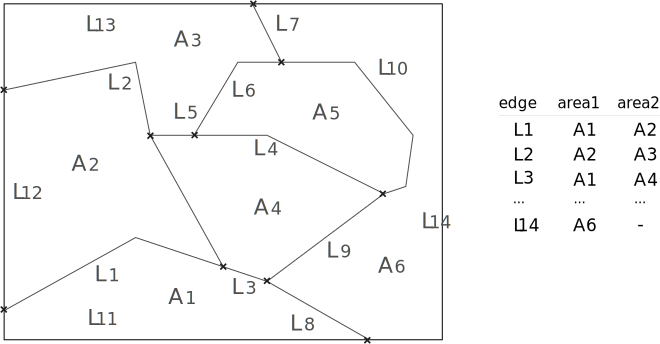
\includegraphics[width=0.7\textwidth]{graphics/basics/topological_vector_model}
  \caption{An example of a topological vector model and an adjacancy table}
  \label{fig:topological_vector_model}
\end{figure}

The topological vector model has a great asset: if an edge between two adjacent areas changes, the connectivity and adjacency does not change and therefore also the topology stays constant. The lookup for neighboring areas is very fast if the topology ensures strict connectivity: The neighbors of an area can be found in the adjacency table. Potentially problematic is the creation of a clean geometry: it can be cumbersome and require a lot of manual adjustment, for example ensuring strict connectivity by manually connecting nodes.

% subsubsection geospatial_topology (end)

% subsection representation_of_space (end)

% ------------------------------------------------------------------------------
\subsection{Representation of Time} % (fold)
\label{sub:representation_of_time}

Unlike in space, time knows only one dimension, which makes modelling simpler. Time is represented by timestamps, with a certain granularity (year, month, day, hour, minute, second, millisecond).

However, there are several different types of time. The simplest categorization is between a discrete \emph{event} and a continuous \emph{process}. Events can happen at a certain \emph{time point} or like processes in a \emph{time interval} or \emph{time period}, defined by two time points. An information system that stores events with a significant outcome regarding the geo-objects in the system, is an \emph{event-based historical geographic information system}. On the other hand, a \emph{process-based historical geographic information system} models mainly processes as a series of events of one kind regarding a small set of geo-objects
\cite[chapter 2, pp. 47-49]{solana2014spatio}.

When storing time related information in an information system, it is furthermore important to distinguish between the time that was true in reality (\emph{valid time} or \emph{world time}) and the time it was stored in the database (\emph{transaction time} or \emph{database time})
% \cite Jensen et al. 1993
\cite[p. 69]{ott2001time}.

The Taxonomic Model of Time by
\cite{frank98typesoftime}
classifies time not only into discrete and continuous, but also by the ``nature of time'': a consecutive development on the time axis, defined by start and end, defines \emph{linear time}. In a contrary, \emph{cyclic time} has no predefined order and events reoccur on a regular cyclic basis.

\paragraph{Temporal Topological Relations} % (fold)
\label{par:temporal_relations}

The topological relationship between two time points $t_1$ and $t_2$ is straightforward. Since they are discrete elements and therefore isomorphic to the space of integers, there are three different order onsrelations:
\begin{compactenum}
  \item $t_1 < t_2$: the first event happens before the second event
  \item $t_1 > t_2$: the first event happens after the second event
  \item $t_1 = t_2$: the first and the second event happen at the same time
\end{compactenum}

For time spans, there are six possibile temporal topological relations (table \ref{tab:temporal_relations}). Except for \texttt{equals}, each of them has an inverse, yielding a total of 13 different relations.

\begin{table}[H]
\begin{center}
\begin{tabular}{c c c}
    \toprule
    relation & symbol & visualization \\
    \midrule
    $X$ before $Y$ &    \texttt{X < Y} & \raisebox{-0.25\height}
    {
\includegraphics{graphics/basics/temporal_relations/before}} \\
    $X$ meets $Y$ &     \texttt{X m Y} & \raisebox{-0.25\height}
    {\includegraphics{graphics/basics/temporal_relations/meets}} \\
    $X$ overlaps $Y$ &  \texttt{X o Y} & \raisebox{-0.25\height}
    {\includegraphics{graphics/basics/temporal_relations/overlaps}} \\
    $X$ equals $Y$ &    \texttt{X = Y} & \raisebox{-0.25\height}
    {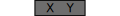
\includegraphics{graphics/basics/temporal_relations/equals}} \\
    $X$ starts $Y$ &    \texttt{X s Y} & \raisebox{-0.25\height}
    {
\includegraphics{graphics/basics/temporal_relations/starts}} \\
    $X$ during $Y$ &    \texttt{X d Y} & \raisebox{-0.25\height}
    {
\includegraphics{graphics/basics/temporal_relations/during}} \\
    $X$ ends $Y$ &      \texttt{X e Y} & \raisebox{-0.25\height}
    {
\includegraphics{graphics/basics/temporal_relations/ends}} \\
    \bottomrule
\end{tabular}
\caption{Temporal relations of time spans}
\small{based on \cite{allen84theoryofactionandtime}}
\label{tab:temporal_relations}
\end{center}
\end{table}


% paragraph temporal_relations (end)

% subsection representation_of_time (end)

% section modelling_time_and_space (end)

% ------------------------------------------------------------------------------
\section{Spatio-Temporal Data Models} % (fold)
\label{sec:spatio_temporal_data_models}

\begin{quoteit}
  ``Geography differs from geometry because \\
  in geography, space in indivisibly coupled with time''
\end{quoteit}
\hfill -- Don Parkes \& Nigel Thrift (1980)

The goal of a HGIS is to show the development of geo-objects over time. Developments are driven by \emph{changes} to the state of an object. According to the Triadic Framework time, space and attribute can change independently from each other. However, in order to trace spatial and attribute changes over time, there has to be a relation between the dimensions.

Abstractly speaking, a goe-object is an \emph{entity} in the information system. Throughout its lifetime, it appears at some point, it might undergo several changes and might disappear at some other time point. The critical point is to maintain the identity of the object: when does an entity change its identity? What kind of changes can occur to an entity without changing its identity, e.g. a name change, a spatial transformation or a splitup.

There are mainly two kinds of changes: \emph{Discrete changes} are based on the idea of a \emph{state machine}: An entity stays in its state until an event occurs that suddenly changes the state at a discrete time point. As an example, the age of human beings changes once per year or their birthday. On a contrary, an entity can gradually change according to a \emph{continuous change}, either in a uniform or a irregular manner. Its development is driven by a process, e.g. the melting of the polar ice caps
\cite{peuquet99}.

Research in the previous 30 years has developed several models for temporal developments of spatial objects with additional attributes. They differ mostly in the main organizing dimension: In \emph{location-based} representations time is an attribute of each geo-object in the systen. \emph{Time-based} models on the other hand explicitly represent events and processes that change geo-objects in the system at a certain time point or in a certain time period.

The basis for all models is the concept of \emph{Time Geography} by
\cite{haegerstrand1970}: Hägerstrand argued for an orthogonal relationship between time and space and that each object can be at one location only at one time. He furthermore visualized an objects development in a \emph{space-time path}. This section will introduce the most important \emph{spatio-temporal data models} (STDM) based on this idea that are releveant for the remaining parts of the thesis.

% TODO: version management (Wachowitz p 43)

% ------------------------------------------------------------------------------
\subsection{Snapshot Model} % (fold)
\label{sub:snapshot_model}

One of the simplest, oldest and most frequently used data model is based on the idea of \emph{snapshots}: At a certain time point $t_i$, a new layer gets created. It stores the full picture of the current state of all geo-objects
\cite{Langran1988frameworktgis}.

\begin{figure}[H]
  \centering
  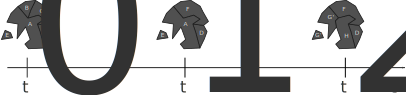
\includegraphics[width=0.8\textwidth]{graphics/basics/stdm/snapshot_model}
  \caption{The Snapshot Model}
  \label{fig:snapshot_model}
\end{figure}

Whereas this model allows to easily retrieve the state of the system at a defined time point $t_i$, it is also its biggest limitation: for all other time points $t \neq t_i$ that are not covered by a snapshot, it is impossible to retrieve the state of the system, because the data model does not record any changes. Additionally, the model is redundant, because objects that have not changed from one snapshot to the next one are duplicated. Although there have been improvements made regarding redundancy in the snapshot model (e.g. \cite{armenakis92}), the main problem that there is no information about the state between two snapshots is integral to the model and can not be solved.

Because of their analogy to photography, snapshots are used e.g. to see the history of a city based on aerial photographs at different time points.

% subsection snapshot_model (end)

% ------------------------------------------------------------------------------
\subsection{Simple Time-Stamping} % (fold)
\label{sub:simple_time_stamping}

Another location-based method is to extend the model for a geo-object by the period of existance. This is done by two more attributes: a \emph{start date} $t_{start}$ at which the object gets created and the \emph{end date} $t_{end}$ at which it is ceased. An object that still exists gets a special value like \texttt{NOW} as a cessation date
\cite{hunter90timestamping}.

\begin{figure}[ht]
  \centering
  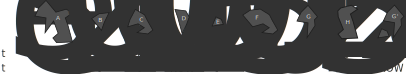
\includegraphics[width=0.8\textwidth]{graphics/basics/stdm/simple_time_stamping}
  \caption{The Simple Time-Stamping method}
  \label{fig:simple_time_stamping}
\end{figure}

This \emph{Simple Time-Stamping} method allows to track changes of objects. Given full and consistent information, the full state of the system at each time point $t_i$ can be retrieved: All geo-objects for which ~$t_{start} \leq t_i < t_{end}$~ are active, all others are inactive. This method works only well for discrete changes. One problem of the model is that it does not allow to trace the development of an entity in different states. If one geo-object ceases and another one starts at the same point, they are visually successors, but this relationship is not implemented in the data model. Whereas this shortcoming can be resolved by adding a reference to the predecessor and the successor of an entity, another disadvantage can not:

It is impossible to say what has happened at a certain time point: If at time point $t_2$ the geo-objects $B$ and $C$ cease and $G$ starts, it could be that they have been unified ($B+C \to G$) or that two are successors ($B \to G$) and one just happens to stop existing without any successor ($C \to \emptyset$). The model is also slightly redundant, because the end date of one geo-object is the start date of another geo-object, if they are historically related. Therefore, in a domain with predecessor-successor-relationships, this model is not very suitable
\cite[p. 46-47]{solana2014spatio}.

Wheresas retrieving a state at a certain time point is possible, it is also cumbersome, because without intelligent data structures every time the date changes, it has to be checked for each geo-object if its state has changed.

% subsection simple_time_stamping (end)

% ------------------------------------------------------------------------------
\subsection{Event-Based Spatio-Temporal Data Model} % (fold)
\label{sub:event_based_spatio_temporal_data_model}

A time-based approach addresses exactly those shortcomings: They explicitly represent events or processes in the data model and associate all entities that change according to them. One example of this approach is the \emph{Event-Based Spatio-Temporal Data Model} (ESTDM) for geospatial raster data by
\cite{peuquet95}.

At one defined time point $t_b$, the \emph{base map} in form of a snapshot gets stored. From that moment on events, the organizing entity of the data model, are stored that change the current status of the map. An event has a time stamp $t_i$ and a list of components associated with it. A component indicates which raster cells (\texttt{x}, \texttt{y}) change their state to a new value (\texttt{v}). The events are chronologically ordered and stored in a doubly-linked event list. Each event knows its preceding (\texttt{prev} pointer) and succeeding (\texttt{next} pointer) event. The data structure furthermore consists of a header file with information about the thematic domain of the model, a pointer to the base map and to the first and last element of the event list.

% TODO: graphic

If the time point of an event is reached, all its event components are executed. The system follows the \texttt{next} pointer to know which event is waiting to be executed next. Since a change is relative to the previous change, not to the base map, change tracking is efficient.

Just like the Simple Time-Stamping method, this approach is only suitable for discrete but not for gradual changes. This problem is addressed in the \emph{ObjectOriented geomorph} model by \cite{raperlivingstone95}.

However, the main constraint for this thesis is that the authors have developed this model only for raster data and have explicitly stated that ``The design of such a [vector-based] model is not seen as a straightforward task'', because of the problem ``how to maintain the integrity of spatial topology as it changes [...] The solution will require a more complex definition of components within individual events''
\cite[p. 21]{peuquet95}.

% subsection event_based_spatio_temporal_data_model (end)

% ------------------------------------------------------------------------------
\subsection{Three-Domain Model} % (fold)
\label{sub:three_domain_model}

The main problem of an event-based STDM for vector geometry including lines and polygons is handle the identity of a geo-object and its spatial, topological and attribute properties throughout the evolution
\cite{yuan96temporal}.

This problem is addressed in the \emph{Three-Domain Model} by \cite{yuan96threedomain}, an approach that handles the three domains of a spatio-temporal object separately:
\begin{compactitem}
  \item The \emph{semantic domain} holds an entity uniquely identifiable. An object in the semantic domain corresponds to a human concept independently from its spatial and temporal properties, e.g. a ``country'', and stores non-spatial and non-temporal attributes of the entity.
  \item The \emph{spatial domain} represents geospatial objects in a vector representation, e.g. a polygon describing the territory of a country.
  \item The \emph{temporal domain} stores all temporal objects, e.g. time points of events, or time intervals of processes.
\end{compactitem}

The model is not specific, but more a general abstract framework to handle space, time and identity. This makes the model very flexible, e.g. it can handle discrete and continuous changes, relative and absolute time, world and database time.

% subsection three_domain_model (end)

% ------------------------------------------------------------------------------
\subsection{History Graph Model} % (fold)
\label{sub:history_graph_model}

Most of the data models introduced so far cover only static changes of geo-objects. \cite{key} identified three different types of temporal behaviour of changing objects:
\begin{compactitem}
  \item Dynamic objects that change continuously.
  \item Static objects that change according to events with duration.
  \item Static objects that change according to sudden events.
\end{compactitem}

Based on this observation he developed a data model that can handle all three kinds of temporal behaviour: The \emph{History Graph Model}. It manages objects and events separetly from each other. An object can only be in three different states:
\begin{enumerate}
  \item An object is \emph{static}, if it currently does not change. This is called an \emph{object version}. The version has an interval associated to it representing the duration of the object version, until it changes the next time. If the object is dynamic and changes continuously, the duration is zero.
  \item If an object is currently \emph{changing}, it is in an \emph{object transition}. The transition has an associated interval as well, whose duration is zero if it is a sudden change. Additionally, a transition links the relevant objects to each other creating temporal predecessor-successor-relationships.
  \item An object that is currently not active, is \emph{ceased} and not visible on the map.
\end{enumerate}

The history of a geo-object is a chronologically ordered set of versions and transitions, that can be visualized in a graph (see figure \ref{fig:history_graph_model}).

\begin{figure}[ht]
  \centering
  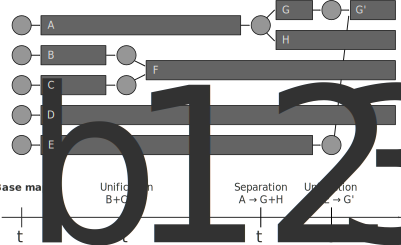
\includegraphics[width=0.8\textwidth]{graphics/basics/stdm/history_graph_model}
  \caption{The History Graph model}
  \label{fig:history_graph_model}
\end{figure}

Renolen defines six basic types of temporal changes that can happen (see figure \ref{fig:history_graph_changes}):
\begin{description}
  \item[Creation]           A new object is created.
  \item[Alteration]         A property of an object (e.g. geometry) changes.
  \item[Cessation]          An object is ceased.
  \item[Reincarnation]      An object that has previously been ceased is recreated.
  \item[Split/Deduction]    An object is divided into two or more new objects or one or more objects are deducted from an existing one.
  \item[Merge/Annexation]   Two or more objects are joined together to a new object or one or more objects are annexed to another object.
\end{description}

\begin{figure}[ht]
  \centering
  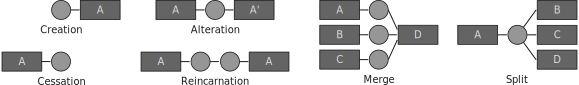
\includegraphics[width=0.8\textwidth]{graphics/basics/stdm/history_graph_changes}
  \caption{Types of changes in the History Graph model}
  \label{fig:history_graph_changes}
\end{figure}

The History Graph model can be seen as an extension to the ESTDM. It combines the advantages of event-based and entity-based spatio-temporal data models, supports discrete and continuous changes and relative and absolute time. But the biggest asset is that the historical development of geo-objects can directly be derived from the model, because objects are linked to their precedessors and successors. The History Graph model can tell a story.

% subsection history_graph_model (end)

% ------------------------------------------------------------------------------
\subsection{Spatio-Temporal Object-Oriented Data Model} % (fold)
\label{sub:spatio_temporal_object_oriented_data_model}

2D geometries + 1D time
element: spatio-temporal atom
event-based: new event => new ST atom stacked on top of existing ones
% \cite Worboys 1992

% subsection spatio_temporal_object_oriented_data_model (end)

%%%%%%%%%%%%%%%%%%%%%%%%%%%%%%%%%%%%%%%%%%%%%%%%%%%%%%%%%%%%%%%%%%%%%%%%%%%%%%%%


implementation
  Spatio-Temporal Data Type (STT)
    time not as an attribute of space -> special entity
    spatio-temporal object model (everything is an object)
      separate classes for Space and Time
      -> aggregation to SpatioTemporal class
      each object with temporal and spatial extension (start + end date, full geo)
    operators for time and space
    time in YYY-MM-DD (ISO 8601 standard)
      `NOW' = still existing = no end date
    \cite{raza12}

other STDM (just to mention)
  Space-time composite
  The grid model
  Amendment vector model
  cell tuple-based spatiotemporal data model
  \cite[p. 14]{zhao11}

% section spatio_tempora_data_models (end)


% ==============================================================================
\section{System Components} % (fold)
\label{sec:system_components}

HGIS like any other system four components
trallala und hoppsassa

% ------------------------------------------------------------------------------
\subsection{Input} % (fold)
\label{sub:input}

Spatial Data for a GIS can either be acquired from existing sources or retrieved manually. One of the most exhaustive collections of geographic data in public domain is hosted by Natural Earth
\footnote{
  \textit{Natural Earth},
  URL: \url{http://www.naturalearthdata.com/downloads/},
  last access: 30.10.2015
}.
There is physical data (e.g. coastlines, rivers, or glacier areas) and cultural data (e.g. political borders, cities, roads, airports or timezones). OpenStreetMap also opens its database to the public
\footnote{
  \textit{Planet OSM},
  URL: \url{http://planet.openstreetmap.org/},
  last access: 30.10.2015
}.
Additionally there is free geodata for special purposes, like regions or statistical data for the USA
\footnote{
  \textit{Free GIS Data - GIS Data Depot},
  geocommunity,
  URL: \url{http://data.geocomm.com/catalog/index.html},
  last access: 30.10.2015
}
or terrain models and administrative regions for Germany
\footnote{
  \textit{Dienstleistungszentrum des Bundes für Geoinformation und Geodäsie},
  Geodatenzentrum,
  URL: \url{http://www.geodatenzentrum.de/geodaten},
  last access: 30.10.2015
}.

% subsection input (end)

% ------------------------------------------------------------------------------
\subsection{Management} % (fold)
\label{sub:management}

Database Management Systems

Version Management
  database has to be updates when change occurs
  versioning methods
    relation-level versioning
      rollback: new event -> new snapshot
      type of change (added, altered/updated, deleted, restored)
    tuple-level versioning
      store changes with event time
      => time slices can be derived from the information about changes
      (+) less redundancy, less data
      (-) weaker performance on retrieval
    attribute versioning
      -> extension of tuple-level versioning: separation entity <-> attribute
      changes stored in attributes
  % \cite Langran 1989

  international boundary has different states:
    event           old b.    new b.              active
    -               valid     -                   old
    legal document  invalid   -                   old
    new demarcation invalid   draft -> invalid    old
    quality control invalid   valid               new
  -> stati: valid, draft, revised, approved = valid
  check on consistency -> only one version accessible to public
  % \cite Wachowicz 1999

Spatio-Temporal Queries


historical R-tree
  assign timestamp t\_i -> active objects = [o\_1, 0\_2, ... , o\_n]
  (+) fast handling of timestamp
  (-) redundancy, because of repeating objects

MV3R tree (Tao \& Papadios, 2001)
  version copy
  (+) less redundant

% ------------------------------------------------------------------------------

A \emph{Database Management System} (DBMS) is a software system for the administration of data, i.e. storage, retrieval, validation of data and their relations. A DBMS has the task to maintain security, performance, stability and allow multi-user access on the same data, following the \emph{client-server} principle.

Data and functions are separated from each other using a \emph{multi-tier architecture} that is best visualized in an example of a Web-based GIS:
% (compare with figure \ref{fig:gis_components}):
The Web browser on the client side hosts the map including content and the tools in the user interface. If the user interacts with a tool the client sends a request to the Web server for new data. The processing layer on the server checks the request and forwards it to the DBMS which translates the request into a query to the database. The result will be handed back to the processor that transforms the data into information and sends it to the client. On the map the new information will be shown.

Following this principle multiple clients can independently from each other get new data from the server, but also multiple processing layers for different purposes can simultaneously request data fro the database, ensured by the DBMS. Another advantage of the clear separation between the data (\emph{model}), the user interface (\emph{view}) and the processing layer (\emph{controller}) follows directly from the \emph{model-view-controller pattern}: One part can be changed without interfering the other parts, e.g. if the map interface changes, the data can stay untouched and an implementation of a new database technology has no consequences to the interface.

There are mainly two types of DBMS: the most common \emph{relational} database and \emph{object-relational} databases that are inspired by the features of object-oriented programming paradigms. Pure \emph{object-oriented} databases will not be covered in this section.

% ------------------------------------------------------------------------------
\paragraph{Relational databases} % (fold)
\label{par:relational_databases}
Databases are built around logical entities that have a discrete set of attributes associated with them, e.g. a city (entity) has a name, a location, a major, a state it belongs to etc. For each member of the entity there is one value for each attributes (e.g. the name of the city is Weimar) which is of a certain data type (integer, decimal, string, boolean, etc.). Entities is a database are represented in a table with rows (one row per member), columns (one column per attributes) and cells (attribute value for this member). Each entity has one attribute that unambiguously identifies each record in the table, the \emph{primary key}.

In a \emph{Relational Database Management System} (RDBMS), entities can be related to each other by three types of relations:
\begin{enumerate}
  \item If each member of one entity has directly one member from another entity associated, it is a direct attributional relation (\emph{1:1}), e.g. each city has exactly one major.
  \item If each member can have several members of another entity related to it, there is a one-to-many (\emph{1:n}) relationship, e.g. each state can have many cities, but a city can only be in one state.
  \item If multiple members from one entity can be related to multiple members of another entity, it is called many-to-many relation (\emph{m:n}), e.g. each river can flow through several states and each state can have several rivers.
\end{enumerate}
The relations are implemented via their primary keys. Many-to-many relationships require another connection table that uses the primary keys from both entities as \emph{foreign keys} in the new table and links them, e.g. if river \texttt{r} flows through countries \texttt{x} and \emph{y}, the connection table would have one record linking \texttt{r} to \texttt{x} and one linking \texttt{r} to \texttt{y}. The entities and their relations are visualized in an \emph{entity-relationship model} (E-R model), as seen in figure \ref{fig:er_example}.

\begin{figure}[ht]
  \centering
  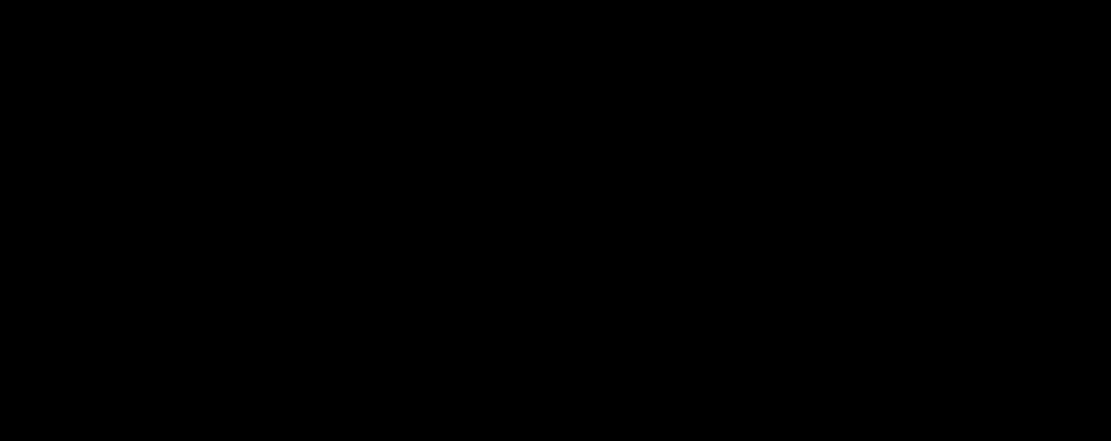
\includegraphics[width=0.75\textwidth]{graphics/basics/er_example}
  \caption{Example for a simple entity-relationship model.}
  \label{fig:er_example}
\end{figure}

Data can be retrieved from a database using the \emph{Structural Query Language} (SQL). An example query to get the names of cities from the state \texttt{Thüringen} in alphabetical order is:
\begin{verbatimtab}
  SELECT     city.id, city.name
  FROM       (city JOIN state ON city.state = state.id)
  WHERE      state.name = ``Thüringen''
  ORDER BY   city.name
\end{verbatimtab}

SQL can also be used to add or manipulate data in a database, e.g. with the \texttt{CREATE} or \texttt{INSERT INTO} commands.

The main goals for each database user is to maintain its correctness,consistency and simplicity and to reduce redundancy in the data. This can be achieved by \emph{normalizing} the database:
\begin{enumerate}
  \item To free the collection of relations from undesirable insertion, update and deletion dependencies.
  \item To reduce the need for restructuring the collection of relations, as new types of data are introduced, and thus increase the life span of application programs.
  \item To make the relational model more informative to users.
  \item To make the collection of relations neutral to the query statistics, where these statistics are liable to change as time goes by.
\footnote{
  \textit{Further Normalization of the Data Base Relational Model},
  E.F. Codd,
  [p. 34]
}
\end{enumerate}

Two examples for RDBMS are \emph{MySQL}, the ``the world's most popular open source database''
\footnote{
  \textit{MySQL :: About MySQL},
  URL: \url{https://www.mysql.com/about/},
  last access: 31.10.2015
}, and the serverless, zero-configuration library \emph{SQLite}
\footnote{
  \textit{SQLite Home Page},
  URL: \url{https://www.sqlite.org/},
  last access: 31.10.2015
}.

% paragraph relational_databases (end)

% ------------------------------------------------------------------------------
\paragraph{Object-relational databases} % (fold)
\label{par:object_relational_databases}

Relational databases are well-suited to manage data in simple form without complex database user requirements. However, there can be more difficult queries to the database. Given the example in figure \ref{fig:er_example}, a user would like to know all rivers that are in and close to the state \texttt{Thüringen}, i.e. they smallest distance between the river and the state border is less than 50 km. A query for that request should look like this:
\begin{verbatimtab}
  SELECT    river.name
  FROM      (river JOIN state JOIN state_rivers)
  WHERE     state_rivers.state = state.id AND
            state_rivers.river = river.id AND
            state.name = ``Thüringen'' AND
            distance (state.location, river.location) < 20
  ORDER BY  city.name
\end{verbatimtab}

This query needs to call the function \texttt{distance}, but user-defined functions are not part of SQL. Also, the data type of the attribute \texttt{location} is not simple: it is not a single value, but rather a \texttt{polyline} or a \texttt{polygon}. Complex user-defined data types are also not integrated in SQL.

ORDBMS behave like RDBMS but can handle complex data. For that matter functionality from object-oriented programming are added, so it supports user-defined data types and functions and the principles such as \emph{encapsulation} or \emph{inheritance}.
% scheiße hier... ich habe keinen Bock mehr jeden Mist hier theoretisch zu erklären. Nur darauf eingehen, wenn ich es wirklich später benutze.
%Encapsulation is the ability make the internal state of an object unaccessible to the outside. Whereas it will be possible to get the coordinates of the location of a city with a simple function it will not be possible to change it directly but through a function \texttt{point.} A request for the perimeter of a  of an object and just give the necessary :
One famous example for object-relational databases is \emph{PostgreSQL}, ``the world's most advanced open source database''
\footnote{
  \textit{PostgreSQL: About},
  URL: \url{http://www.postgresql.org/about/},
  last access: 31.10.2015
}.

% ------------------------------------------------------------------------------
\paragraph{Spatial databases} % (fold)
\label{par:spatial_databases}
GIS can deal with a lot of coordinate data. This amount of data has to be processed efficiently in order to maintain a good overall system performance. \emph{Spatial databases} are specialized for this matter. They have predefined data types such as \texttt{point}, \texttt{polyline} or \texttt{polygon} and support spatial queries such as functions to solve the point-in-polygon problem or to calculate a distance between two polylines. \emph{PostGIS} is an extension for PostgreSQL that is especially utilized for GIS
\footnote{
  \textit{PostGIS},
  URL: \url{http://postgis.net/},
  last access: 31.10.2015
}.
\emph{SpatiaLite} is a library for the same purpose, extending SQLite's relational database management system
\footnote{
  \textit{SpatiaLite},
  URL: \url{https://www.gaia-gis.it/fossil/libspatialite/index},
  last access: 31.10.2015
}.

% paragraph spatial_databases (end)

% ------------------------------------------------------------------------------
\paragraph{Spatio-Temporal Databases} % (fold)
\label{par:spatio_temporal_databases}

how to store and query spatial and temporal data?

static databases
  no updates, old information overwritten by new information
  -> not suitable for spatio-temporal object management
static rollback approaches
  implementation of relation-level versioning
  change -> copy old data, change elements to new data => complete new time slice
  (+) effective versioning
  (+) fast retrieval of state at time point x
  (-) highly redundant
historical databases
  store valid state at a specific time point (valid time)
  store time slices valid for specific time steps
  or validity of objects between events
  -> changes only made with valid time
temporal databases
  support both valid and transaction time
  retrieval of current state at given time step
  (+) supports retrieval of what was known to the database at given time point
  usage in knowledge and research database
  usage when different sources for same event are used
  -> supports different views on world

implementation using relational databases
separation time and space in database

ER model for temporal objects
  % \cite Basogly \& Morrison
  example: administrative units
  units change borders and attributes over time
  units valid over certain period of time
  units have ancestors and successors
  -> units gain area from or loose area to one or several other units
  hierarchical structure of units (country -> state -> county -> city -> neighborhood -> ...)
  units can have additional attribute data (e.g. statistics per year)
  % \cite Pierau 1998
  \cite[p. 67-68]{ott2001time}


% paragraph spatio_temporal_databases (end)

% section management (end)

% ------------------------------------------------------------------------------
\subsection{Analysis} % (fold)
\label{sub:analysis}

% TODO: spatio-temporal queries

analysis: determine, change, evaluate

analysis methods
  spatial analysis
  temporal analysis
    time series analysis
    process analysis      (modification modeling + future forecasting)
  attribute analysis
alteration of \cite[p. 128]{ott2001time}

spatial queries
  query of spatial properties and attribute values
  e.g. size of Germany in 1871
thematic queries
  query objects based on certain criteria (spatial and attribute)
  multi-criteria analysis
  e.g. all democratic countries larger than 10.000 km²
statistical analysis
  artithmetic calculation and classification of characteristics of objects
  univariate, multivariate investigation
  e.g. What was the population density in Germany in 1945 compared to 1995
overlay/split
  aggregation and splitting of spatial components based on the layer principle
  e.g. Germany in 1945 gets split up into FRG and GDR by one polyline (inner German border) and one polygon (West Berlin)
geometric-topological operations
  analyze the neighborhood relations between geometric objects
  e.g. is the geometry all countries at time point 1991 strictly connected?
temporal analysis
  using spatial and temporal operators in figure
  %\ref{fig:spatial_temporal_operators}
  e.g. in which year did the largest amount of border changes happen?
\cite[p. 129-140]{ott2001time}

Multivariate Historical-Geographical Model
  multivariate
    features of a spatial object
    connection between temporal development of features
  geographical model
    location (geometry)
    neighborhood relation (topology)
  historical model
    object at different points in times
  \cite[p. 128]{ott2001time}
  % \cite Kilchenmann 1992

Spatial Queries / Operators
  and     intersection
  not     difference
  or      (cascaded) union
  xor     (inverted) symmetric difference

Temporal Queries / Operators

temporal logic
  rules and symbols
  represent time
  reason about time
  temporal operators
  ??? detail?
  % \cite Hodkinson and Reynolds 2006

  trajectories
    sequence of 2D or 3D locations of an object

Spatio-Temporal Queries / Operators
  when + where -> what
  when + what -> where
  where + what -> when
  % \cite Peuquet 1994


% ------------------------------------------------------------------------------
A GIS shall solve the problem for a user or answer his or her research question. Given a well-filled database with a working DBMS, the data might not answer the research question directly. It has to be sorted, selected or classified in order to convey the required information. For this process there are \emph{spatial operations} on the data in the system. Several operations can be applied in a certain order
\cite[pp. 321-325]{bolstad2008gis}.
Both spatial and attribute data are analyzed to combine the dimensions \emph{where?} and \emph{what?} in order to answer the ultimate question \emph{why?} something is the way it is
\cite[p.xii-xvi]{knowles2002past}.

An example is a system visualizing social developments on Earth. The researcher wants to divide the world into five regions with a similar life expectancy to see if there are spatial discrepancy of advances in global health. He or she has a GIS with all countries and their current life expectancy stored. In order to answer his or her research question, the following steps may be required

\begin{enumerate}
  \item Extract the life expectancy value per country.
  \item Classify the values on a discrete scale from very low to very high and put each country into one of the five classes.
  \item Unify neighboring countries that are in the same class to get five world regions.
  \item Name the five world regions.
  \item Apply a color scheme to the classification and set the background color for each of the five world regions.
  \item Create a legend with the classification and the explanation of the symbols.
  \item Present the resulting map on the screen.
\end{enumerate}

There are special operations for raster data, e.g. spatial interpolation, and for vector data.

Only explain those later that are really important!

graph / network analysis
  what is the shortest way from A to B?
  what is the fastest route from A via B1, B2, ..., Bn nack to A? (TSP)

Polygon geometry
  intersection, (cascaded) Union, (symmetric) difference

Polygon Clipping
  Sutherland-Hodgeman
  Weiler-Atherton

Topology analysis
  test for consistency, connectedness and completeness of topology

% subsection analysis (end)

% ------------------------------------------------------------------------------
\subsection{Presentation} % (fold)
\label{sub:presentation}

spatio-temporal visualization
-----------------------------

spatial domain
  2D: map, different projections
  3D: globe

temporal domain
  linear time
    time line
    time series: graph (t,y coordinate system)
    2.5D map: temporal dimension on z axis or on surface
    space-time path
  cyclic time
    time series: polar diagram
    time wheel
  both
    mono-temporal: one layer -> one time point
    multi-temporal: one layer -> multiple time points
\cite[p. 144]{ott2001time}

direct display of time on a map
  choropleth maps
  temporal diagrams
  change indicators

display mechanisms for visualizing temporal change
  change data         additional to base map (diagrams, texts)
  static symbols      thematic map, symbols: dates, routes, developments
  time sequence maps  mono-temporal maps in sequence
  animations          interactive visualization of time and space and attributes
\cite[p. 146-147]{ott2001time}


other approaches
  scatterplot               variation of two variables over time
  parallel coordinate plot  variation of multiple variables over time
  time series graph         variation of one variable over time

visualization in a way that people can understand it
  self-organizing map (SOM) nD variables -> 2D space + 2D color scheme
  % \cite Guo et al 2006


Scivis vs. Infovis

list of all possible spatial presentations -> only focus on maps
list of all possible temporal presentations -> only focus on timelines

Cartographic visualizations are the interface between the GIS and the human. A map is is the common form. It is a discrete graphical expression of the continuous real world. The creation of a map is not just a scientific, but also a creative process: The form, function and interaction methods shall follow the purpose of the usage of the map.

There is no fixed guideline how to properly design a map, but there are typical elements that are part of every cartographic visualization.The main element is the map itself, using a specific map projection
% (see section \ref{ssub:map_projections})
, a scale and an initial center point. A map is typically structured in a \emph{layer} principle. Each layer is a transparent film showing one specific aspect, e.g. a physical layer showing coastlines, mountains or forests, a political layer showing international borders or a cultural layer showing cities or population densities. The layers are interchangeable, can be switched on and off and serve to serve a different visualization purpose. The map is designed using a certain color scheme, fonts and signatures for all the objects on the map.

Additionally there can be a \emph{title} describing the purpose of the map. A \emph{legend} including the scale bar and north arrow shall explain all symbols used on the map and give orientation. Depending on the degree of interactivity, there can be \emph{menus} with different visualization options, e.g. panning and zooming on the map, switching map layers on and off or changing the color scheme of the map.
\cite[pp. 159-166]{bolstad2008gis}

% example of a good map

The main goal of map design is to give the user nothing but the necessary information he needs to satisfy his or her information need. The cartographer shall use techniques of \emph{cartographic generalization} to minimize information on the map and maximize the knowledge to be extracted from the map. Simplification, smoothing or aggregation help to reduce amount of information. Enlarging, widening or displacement help to focus on the important areas of the map. Selection and classification help the user to get an overview of the information.
\cite{krygier2005making}

Leaflet.js is ``an open-source JavaScript library for mobile-friendly interactive maps''
\footnote{
  \textit{Leaflet - JavaScript library for interactive maps},
  URL: \url{http://leafletjs.com/},
  last access: 02.11.2015
}
that offers functionality to embed a map with a chosen projection in an HTML document, use own map tiles, symbols and markers on the map and tools for zooming and panning.
The same service is provided by \emph{OpenLayers}, a ``A high-performance, feature-packed library for all your mapping needs''
\footnote{
  \textit{OpenLayers 3 - Welcome},
  URL: \url{http://openlayers.org/},
  last access: 02.11.2015
}, just with more features and users.


% ------------------------------------------------------------------------------
\subsubsection{Maps} % (fold)
\label{ssub:maps}


maps are means and products of GIS

scientific visualization vs. information visualization
  tangible objects            abstract concepts
  with inherent form          without inherent form
  e.g. CT scan of human body  e.g. flow of refugees
-> 3D globe: inherent form, direct representation of Earth -> scientific visualization
-> 2D map and time: no inherent form resp. abstract concept
=> information visualization

tasks of visualization
  present (what? where? when? how?)
  analyze (e.g. what is the best? where is the most? when was the first?)
  explore (why?)
% \cite Kraak 1999

interactive map enhances human cognition (panning, zooming, changing map layers, time point, data source, ...) and lets him gain knowledge about the domain

maps contain symbols and elements
  ... blaaa ...

traditional paper maps vs. modern digital maps
\begin{table}[ht]
\centering
\begin{tabular}{llp{1em}ll}
    \toprule
    \multicolumn{2}{c}{classical map} & & \multicolumn{2}{c}{modern digital map} \\
    character & restriction & & character & improvement \\
    \midrule
    static & only discrete point in time & & dynamic & higher sample rate for continuous processes \\
    isolating & only part of geographical space in 2D & & multi-dimensional & multiple levels of detail, possibility for representation of elevation and temporal dimension \\
    selective & only one layer & & inclusive & change layers and perspectives \\
    passive & only sending information & & interactive & direct manipulation and exploration \\
    \bottomrule
\end{tabular}
\caption{Innovation of modern digital maps}
\small{alternation of \cite{karcher} and \cite[p. 145]{ott2001time}}
\label{tab:maps_restrictions}
\end{table}

modern digital maps can show changes in time and space due to their dynamic, multi-dimensional, inclusive and interactive nature.


\paragraph{Map Projections} % (fold)
\label{par:map_projections}

Based on the geodetic datum a three-dimensional representation of the Earth in form of a globe would be a possible medium to view the planet. When seen perpendicular onto the world, a globe represents sizes, shapes, distances and directions of objects close to the viewpoint with a reasonable accuracy. However, they are very space-consuming and cumbersome. For a precise measurement of distances, following a route or examining a terrain model, the globe would have to be very large. Therefore, the desired medium for practical purposes is a two-dimensional map.

The basic problem to be solved is that the Earth is a spherical object, its surface is curved and it is therefore not straightforward to project it onto a flat 2D map. The meridians which are lines of equal value converge at the poles. Neighboring meridians (distance: 1\degree) have a distance of 111 km at the Equator and 0 km at the poles. They do not form a right-angled grid with the parallels and therefore no Cartesian coordinate system. This is the reason why the geometries of the spherical Earth will be distorted when displayed on a flat 2D Cartesian coordinate system. \cite[p.79]{bolstad2008gis}

% \begin{figure}[ht]
%   \centering
%   \includegraphics[width=0.66\textwidth]{graphics/basics/distortion}
%   \caption{Distortion visualized by circles on a 2D map as a Cartesian coordinate system}
%   (on the 3D Earth all circles have the same size)
%   \label{fig:distortion}
% \end{figure}

There are two main classifications of map projections: The \emph{projection family} with respect to the geometric shape used for the transformation: \emph{cylindrical}, \emph{conical} and \emph{azimuthal} or \emph{planar projection}). Secondly, the \emph{distortion characteristics} with respect to the map property that is preserved. There are \emph{equivalent}, \emph{conformal}, \emph{equidistant}, \emph{zenithal} and compromise projections. Most families and characteristics can be mixed, e.g. it is possible to create a cylindrical, a conical and an azimuthal equivalent map projection
\cite{mapProjectionKrygier}.


\paragraph{Projection Families} % (fold)
\label{subp:projection_families}

The basis of geometrical map projections are \emph{developable surfaces} onto which the ellipsoidal model of the Earth is projected. The are mainly three geometric shapes that are used as reference surfaces: cylinders, cones and planes. The model is fitted in or on the surface touching it in at least one point or line. The idea is that there is a projection source from which rays are shot through the ellipsoid on the surface, projecting each point of the ellipsoid onto the surface (as seen in figure \ref{fig:projections}). This principle is known from the ray casting technique in computer graphics
\cite{mapProjectionGeokov}.

\begin{figure}[ht]
  \centering
  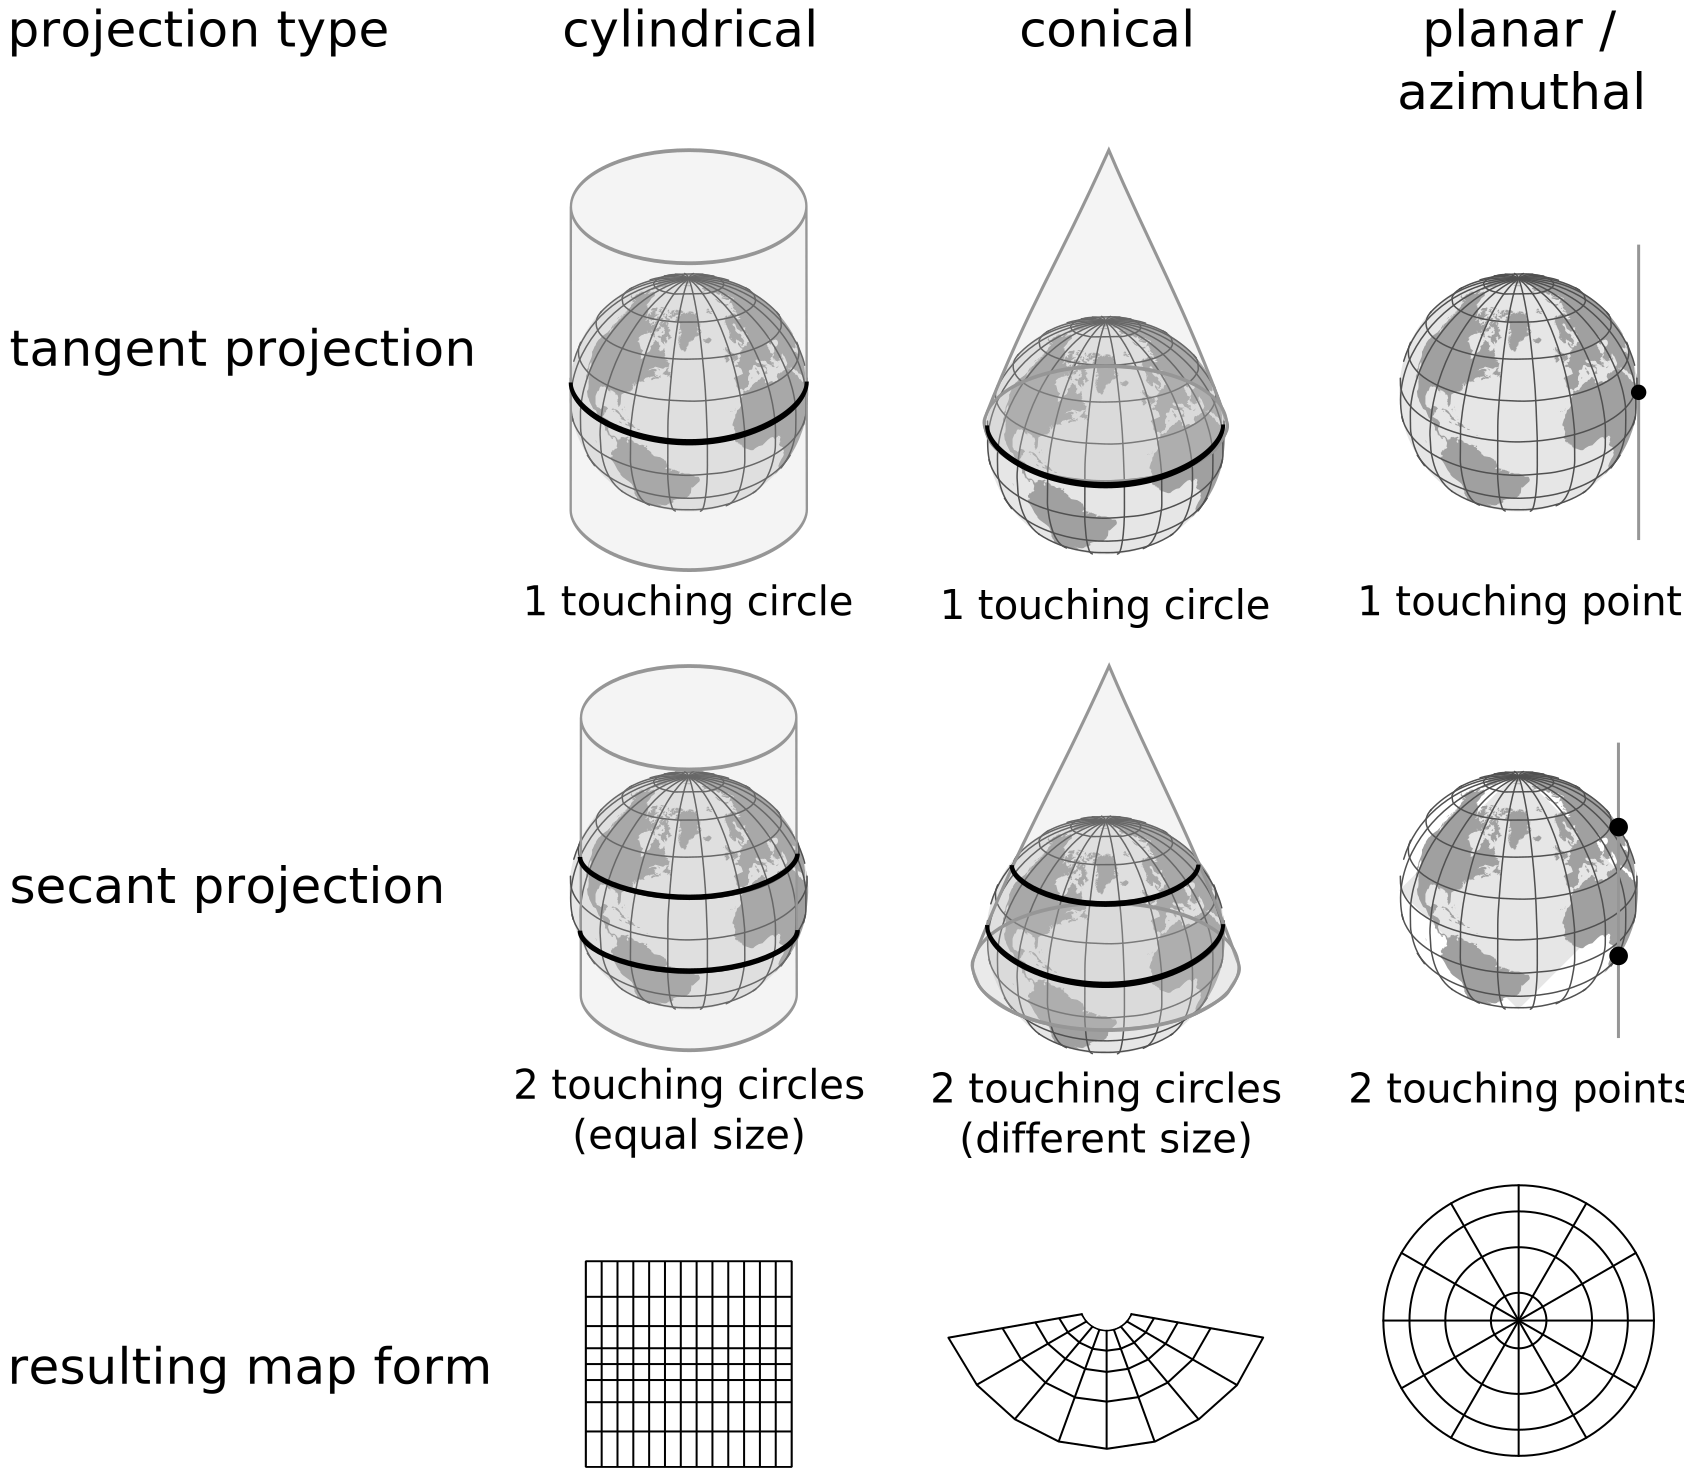
\includegraphics[width=0.73\textwidth]{graphics/basics/projections}
  \caption{Three different developable surfaces for map projections \protect\footnotemark}
  \label{fig:projections}
\end{figure}

\footnotetext{
  based on: \textit{Coordinate Reference Systems},
  QGis Documentation,
  URL: \url{http://docs.qgis.org/2.0/en/docs/gentle_gis_introduction/coordinate_reference_systems.html},
  last access: 27.10.2015
}

In praxis, also pure mathematical map projections are used, e.g. pseudocylindrical, sinusoidal or Mollweise projections. They are much more complex and have the goal to reduce the overall distortion
\cite[p.99]{bolstad2008gis}.

% subsection projection_families (end)


\paragraph{Distortion characteristics} % (fold)
\label{par:distortion_characteristics}

To flatten a spherical surface onto a flat surface, transformations such as stretching, tearing or shearing have to be performed. % affine? non-affine?
A map projection is only accurate at the \emph{standard lines}, i.e. the point(s) or line(s) where the developable surface touches or intersects the ellipsoid. In all other parts the map will in some ways be deformed. That causes distortion in at least one of the following properties of a map: shape (angle), size (area),  direction or distance of features on the map. There is no perfect map projection. Each projection can preserve maximum two of these properties at a cost of distorting the others. The cartographer has to make a compromise and choose a set of characteristics that are important while accepting a distortion in the other properties.

\emph{Tissot's indicatrices} visualize the distortion patterns in the form of ellipses on the map. Their size, shape and orientation are caused by the map projection and show the distortion at this point of the map. Using indicatrices the advantages and disadvantages of each map projection can be shown.

There are two mutual exclusive characteristics: \emph{equivalent} and \emph{conformal}. Equivalent projections preserve the sizes and areas of features on the map, whereas conformal projections preserves angles and the shapes of objects. Every map projection that is area-preserving distorts shapes at the same time, and vice versa
\cite{mapProjectionGeokov}.

\begin{figure}[ht]
  \centering
  \begin{subfigure}{0.59\textwidth}
    \centering
    \includegraphics[width=0.9\linewidth]{graphics/basics/projection_distortion_lambert.png}
    \caption{Lambert cylindrical projection \protect\footnotemark}
  \end{subfigure}
  \begin{subfigure}{0.39\textwidth}
    \centering
    \includegraphics[width=0.9\linewidth]{graphics/basics/projection_distortion_mercator.png}
    \caption{Mercator cylindrical projection \protect\footnotemark}
  \end{subfigure}
  \caption{Comparison of equivalent and conformal map projections}
  \label{fig:lambert_vs_mercator}
\end{figure}

% reset footnotecounter by 1 (for left subfigure caption)
\addtocounter{footnote}{-1}
\footnotetext{
  \textit{Tissot indicatrix world map Lambert cyl equal-area proj},
  Eric Gaba / Sting (Wikimedia), June 2008
  URL: \url{https://commons.wikimedia.org/wiki/File:Tissot_indicatrix_world_map_Lambert_cyl_equal-area_proj.svg},
  last access: 28.10.2015
}

% set footnotecounter to next footnote (for right subfigure caption)
\addtocounter{footnote}{1} % count to next footnote
\footnotetext{
  \textit{Tissot indicatrix world map Mercator proj},
  Eric Gaba / Sting (Wikimedia), September 2008
  URL: \url{https://commons.wikimedia.org/wiki/File:Tissot_indicatrix_world_map_Mercator_proj.svg},
  last access: 28.10.2015
}

The \emph{Mercator projection} (figure \ref{fig:lambert_vs_mercator}b) is an angle-preserving map. It was used for nautical navigation because of a very helpful property: constant compass bearing. A straight line on a Mercator map crosses all meridians in the same angle, a so called \emph{loxodrome}. A navigator only has to follow this line and never needs to reset the compass, because it will always point in the same direction. This is not the shortest way from A to B, but the easiest to navigate. The disadvantage of Mercator maps are the large area distortions towards the poles, which can be seen at the sizes of the ellipses. The best example visualizing the problem is Greenland: On the map it seems almost as large as Africa, whereas in reality Africa is 14 times larger than Greenland.
\cite{mapProjectionGeokov}

This scale becomes obvious in the area-preserving \emph{Lambert projection} (figure \ref{fig:lambert_vs_mercator}a). Tissot's indicatrices all have the same size, but their shapes get distorted towards the poles. This map shows the real size of Africa, but largely distorts the shape of Europe. However, for thematic mapping and teaching purposes equivalent projections are well-suited, because they accurately show the areas of the countries.
\cite{mapProjectionGeokov}

The result of an \emph{equidistant} projection is a map that in relation to the scale accurately shows the distances between certain points on the map.

\vspace{0.5em} % unfortunately necessary to prevent awkward linebreak in footnotes
\begin{figure}[ht]
  \centering
  \begin{subfigure}{0.62\textwidth}
    \centering
    \includegraphics[width=0.9\linewidth]{graphics/basics/projection_distortion_equirectangular.png}
    \caption{Equirectangular equidistant cylindrical projection \protect\footnotemark}
  \end{subfigure}
  \begin{subfigure}{0.37\textwidth}
    \centering
    \includegraphics[width=0.9\linewidth]{graphics/basics/un_logo}
    \caption{Logo of the United Nations \protect\footnotemark}
  \end{subfigure}
  \caption{Two examples of equidistant map projections}
  \label{fig:equidistant_projections}
\end{figure}

% reset footnotecounter by 1 (for left subfigure caption)
\addtocounter{footnote}{-1}
\footnotetext{
  \textit{Tissot indicatrix world map equirectangular proj},
  Eric Gaba / Sting (Wikimedia), June 2008
  URL: \url{https://commons.wikimedia.org/wiki/File:Tissot_indicatrix_world_map_equirectangular_proj.svg},
  last access: 28.10.2015
}

% set footnotecounter to next footnote (for right subfigure caption)
\addtocounter{footnote}{1} % count to next footnote
\footnotetext{
  \textit{Logo of the United Nations},
  Shizhao (Wikimedia), 13.06.2007
  URL: \url{https://commons.wikimedia.org/wiki/File:Logo_of_the_United_Nations_(B\%26W).svg},
  last access: 28.10.2015,
  Comment: This work is excerpted from an official document of the United Nations prior to 17. September 1987.
}

% pidgeon
% irc.freenode.net#slab

Figure \ref{fig:equidistant_projections}b shows a prominent example: The Unites Nations chose a map for their logo from which all points on the map have the correct distance to the North Pole. The equirectangular projection in Figure \ref{fig:equidistant_projections}a has a slightly different property: any meridian is true to scale and therefore all distances along the meridians are accurate. However, the ellipses on the map are distorted in both shape and size, so the map is neither conformal nor equivalent. Air navigation charts or seismology make use of the equidistant property e.g. to show distances from major cities to the epicenter of an earthquake.
\cite{mapProjectionGeokov}

\emph{Zenithal} or \emph{azimuthal} projections preserve directions from the center point to all other points on the map (see figure \ref{fig:zenithal_projection}). It is only possible in the family of planar projections and can be combined with a conformal, equivalent and equidistant property. These maps are used whenever directional relationships are important, for example in navigational charts.

\begin{figure}[ht]
  \centering
  \includegraphics[width=0.3\textwidth]{graphics/basics/projection_distortion_azimuthal.png}
  \caption{Lambert azimuthal (zenithal) equivalent projection \protect\footnotemark}
  \label{fig:zenithal_projection}
\end{figure}

\footnotetext{
  \textit{Lambert azimuthal equal-area projection SW},
  Strebe (Wikimedia), 15. August 2011
  URL: \url{https://commons.wikimedia.org/wiki/File:Lambert_azimuthal_equal-area_projection_SW.jpg},
  last access: 28.10.2015
}

If no characteristic is explicitly important but the overall distortion shall be minimized, a \emph{compromise projection} can be used. They do not preserve any property, but are a trade-off in the distortion of all other properties. The Robinson projection in figure \ref{fig:robinson_projection} is a well-known example. All Tissot's indicatrices not on the Equator are distorted in size, shape and direction, but compared to the Mercator or Lambert projection, the magnitude of distortion is lower.

\begin{figure}[ht]
  \centering
  \includegraphics[width=0.65\textwidth]{graphics/basics/projection_distortion_robinson.png}
  \caption{Robinson projection \protect\footnotemark}
  \label{fig:robinson_projection}
\end{figure}

\footnotetext{
  \textit{Tissot indicatrix world map Robinson},
  Eric Gaba / Sting (Wikimedia), June 2008
  URL: \url{https://commons.wikimedia.org/wiki/File:Tissot_indicatrix_world_map_Robinson_proj.svg},
  last access: 28.10.2015
}

% paragraph map_projections (end)

% subsubsection maps (end)

% ------------------------------------------------------------------------------
\subsubsection{Timelines} % (fold)
\label{ssub:timelines}

% subsubsection timelines (end)

% subsection presentation (end)

% section system_components (end)

% ==============================================================================
\section{Application} % (fold)
\label{sec:application}

In summary,  The research focuses on changes over time triggered by historical events happening in an historical context. There are currently no historical information systems that scientists of this field use for their research, it is rather based on primary and secondary sources, e.h. historical documents, speeches or photography.

\emph{Historical} or \emph{temporal geographic information systems} (HGIS) combine elements of history and geography into one information system to be able to answer research questions for both historians and geographers: ``situating history in its geographical context and using geographic information to illuminate the past.''
\cite[p. 3]{knowles2008placing}
This manifests the interdisciplinary nature of HGIS and making it also an interesting technology in the context of \emph{digital humanities}, the intersection between humanities and computing. The main distinction to classical GIS is the integration of the component of time, making the system four-dimensional. HGIS collect, manage, analyze and present spatio-temporal information and models changes over time and space
\cite[p. xii]{knowles2002past}

there is ``not any operational temporal GIS''
\cite[p. 5]{raza12}

  \emph{lifelines}
    showing tracks, routes and meetings or people -> linear, time steps
    historic example: Napoleons Moscow Campaign
    \includegraphics[width=0.8\textwidth]{graphics/basics/napoleon_march_moscow.png}
    \footnote{
      \textit{Minard.png}
      Charles Minard, 1869,
      URL: \url{https://commons.wikimedia.org/wiki/File:Minard.png},
      last access: 03.11.2015,
      Charles Minard's 1869 chart showing the number of men in Napoleon’s 1812 Russian campaign army, their movements, as well as the temperature they encountered on the return path. Lithograph, 62 x 30 cm
    }
    \cite[pp. 188-191]{knowles2008placing}

  reason about historical events
    combine spatial and temporal and attributional information -> overlays
    e.g. Battlefield stories (what was the cause for the victory of party A?)

  mapping historical maps (historical status)
    most part of the work: digitizing and systematizing primary source material into spatial and attribute data (geodata)
    -> georeferencing, semi-automatic feature extraction, manual data entry
    \cite[pp. xvii]{knowles2002past}
    There are several techniques to acquire geodata as a primary source, e.g. through surveying, aerial and satellite imaging using remote sensing and photogrammetry
    \cite[p. 148-149, p. 213-216]{bolstad2008gis}.
    Spatial data from a hardcopy map can be gained by a two-step process that can be seen in figure \ref{fig:hibo}:
    First project the map into the coordinate system of the world by \emph{georeferencing}. The result is that each pixel of the raster graphic is assigned a geographic coordinate from the real world, so the geometry is given a spatial reference. Afterwards acquire the coordinates of the desired features on the map through semi-automatic digitizing
    \cite[p. 133-142]{bolstad2008gis}.

    \begin{figure}[ht]
      \centering
      \begin{subfigure}{0.48\textwidth}
        \centering
        \includegraphics[width=0.95\linewidth]{graphics/basics/hibo1.png}
        \caption{Georeferencing}
      \end{subfigure}
      \begin{subfigure}{0.48\textwidth}
        \centering
        \includegraphics[width=0.95\linewidth]{graphics/basics/hibo2.png}
        \caption{Semi-automatic digitizing}
      \end{subfigure}
      \caption{Semi-automatic extraction of a border from a map of the Roman Empire \protect\footnotemark}
      \label{fig:hibo}
    \end{figure}

    \footnotetext{
      \textit{HiBo - semi-automatic extraction of borders from historical maps},
      Project of: B. Weber, N. K. Dankwa, K. Singh and T. Kashyappan, supervised by: Prof. Volker Rodehorst and Marcus Kossatz, Bauhaus-Universität Weimar, February 2015,
      URL: \url{https://bitbucket.org/bastian_weber/hibo},
      last access: 29.10.2015
    }


HGIS projects
  usage: mostly quantitative research
  -> logical characteristics of information system)

  large collection of research projects
  \cite{knowles2008placing}
  \cite{gregory2014toward}

  ``The Barrington Atlas of the Greek and Roman World''
    gazetteer: name of historic place -> map by map
    \cite{talbert2000barrington}
    \footnote{
      \textit{Ancient World Mapping Center},
      The University of North Carolina,
      URL: \url{http://awmc.unc.edu/},
      last access: 03.11.2015
    }
  solution
    think about how to represent historical knowledge in geographic context
    degree of certainty -> ironically: that has to be exact as well in a database table
    => reason: careful conclusions from historical maps
  problem: tedious manual work
    ~20 hour per map already digitized
    \cite[pp. 145]{knowles2002past}

  show change over time (historical development)
  state-based approach (photography: validity period of geometries)

  ``Great Britain Historical GIS Project'' (GBHGIS)
    \footnote{
      \textit{Great Britain Historical Geographical Information System (GBHGIS)},
      Ian Gregory \& Humphrey R. Southall, University of Portsmouth, since 1994,
      URL: \url{http://www.port.ac.uk/research/gbhgis/},
      last access: 02.11.2015
    }
    idea:
      combine statistical data with territorial units
      => new analytical opportunities
      e.g. analyze net migration in the districts in UK
      -> snapshot model
    problem:
      ``To map and spatially analyze data correctly, quantities must be linked to an accurate representation of the units for which they were collected.''
      administrative units / districts fundamentally changed three times and slightly changed hundreds of times over the last 200 years
      statistical data is gathered per unit
      hardly any info about historical boundaries of districts
      (some by British Ordnance Survey, but not covering everything)
      => results would be disproportional
    \cite[pp. 117-129]{knowles2002past}
    solution: aerial interpolation
      geostatistical interpolation
      discrete data proportional to source polygon (old geometry) -> reaggregate to target polygons (new geometry)
      => prediction
      \cite{aerialInterpolation}

    UK ordnance survey
      * automatic change detection
      \url{https://www.ordnancesurvey.co.uk/education-research/research/automatic-change-detection.html}

  ``National Historical Geographic Information System'' (NHGIS)
    \footnote{
      \textit{Welcome to NHGIS},
      Minnesota Population Center, University of Minnesota,
      since 2007,
      URL: \url{http://www.port.ac.uk/research/gbhgis/},
      last access: 02.11.2015
    }
    idea:
      provide digital boundaries for each census year
      -> estimation of population of any year
    concept:
      composite map: each face represents an area that never changed
      -> composition to regions per year based on compositing information
      dealing with problem of varying administrative borders through aerial interpolation
    interface:
      very scientific a lot of options
      need tutorial to go through the selection
      need to register before downloading something
      get a link to download a file
      have to decompress it
      then load it into your preferred GIS
      -> incredibly frustrating !!!


This application does maps and timelines:

https://www.palantir.com/palantir-gotham/applications/

MAP
The Map application delivers geospatial analytic capabilities. It combines the visualization of geo-located objects on a map with histogram, timeline and time wheel visualizations. A heatmap visualization illuminates the density of interesting objects on the map.

The imagery on the Map is fully pluggable, allowing users to switch between different sources of imagery, integrate private imagery, and create composite imagery sets that combine two or more sources of imagery.

KML and Shapefiles can be imported as independent map layers, and shapes contained in these layers can be used to select and filter objects that lie in a similar region (like a county, census plot, or state). Layers can be colored and labeled according to calculations performed on the data they contain.


Here is a group using the tool to do historical maps: http://envisioninghistory.org/


And here is a program I’m using for my dissertation. I don’t know if it does timelines and maps, but I think it might.

http://www.tableau.com/

Here are some examples of what I’m doing with it:
% https://public.tableau.com/profile/ammon.shepherd#!/

And my dissertation website just for fun: http://nazitunnels.org

The major problem that lays in the nature of the qualitative historical research is that all historic sources are subjective and biased, their content may be fuzzy and they are definitely incomplete. So the knowledge that can be extracted from a source bears the integral problem of \emph{uncertainty}. On the other hand there are information systems with a logical architecture, with the goal to be as precise and accurate as possible. Analysis is based on mathematical functions -- in its entire nature an information system is quantitative. This contrast is the main problem why HGIS is not widely accepted yet
\cite[p. 2]{knowles2008placing}.

Another problem for historians is that they do not necessarily need a tool to better visualize existing knowledge (e.g. historical maps), but to generate new knowledge by analyzing spatio-temporal coherences or distributions in historical data. Spatio-temporal reasoning is still an open field and not easily possible with existing HGIS
\cite[p. 268]{knowles2008placing}, \cite[p. xii]{gregory2014toward}.

Some interesting research questions that could be answered using HGIS could be:

\begin{itemize}
  \item Did the European Union help to bring peace on the European continent or the other way around? (political)
  \item Is there a coherence between life expectancy and fertility rate on earth? (social)
  \item Does global warming speed up the melting of the glaciers? (physical)
  \item What was the contribution of Bismarck's foreign policy to a longer period of peace in Europe from 1871 to 1914? (historical)
\end{itemize}

Or on a more abstract level: Where and When has something changed and why did it change?


space-time premise by Gaddis 2002
  time and space equal importance
  event     what significantly has happend and by whom? (singularity!)
  process   how something has happened? (event+activity => trigger of process)
  change    driven by process
  spatiotemporal data defines all above three
  % \cite Gaddis 2002


% ------------------------------------------------------------------------------
\subsection{Digital Humanities} % (fold)
\label{sub:digital_humanities}

% subsection digital_humanities (end)

% ------------------------------------------------------------------------------
\subsection{HistoGlobe} % (fold)
\label{sub:histoglobe}

% subsection histoglobe (end)

% section application (end)


\vspace{2em}

transition to concept chapter